% Chapter Template

\chapter{Evaluation} % Main chapter title

\label{Chapter4} % Change X to a consecutive number; for referencing this chapter elsewhere, use \ref{ChapterX}

\lhead{Chapter 4. \emph{Evaluation}} % Change X to a consecutive number; this is for the header on each page - perhaps a shortened title

To evaluate our solution, we follow two directions. First, we test the fact that our benchmark supports MTC filesystems and that it can measure the metrics described by the MTC Envelope. Second, we observe whether our project is easier to use than the current benchmarking solutions for MTC filesystems.

To assess the first part, we ran the following benchmarks on the two discussed MTC filesystems - MemFS and AMFS.

\begin{itemize}

\item 1-to-1 read
\item N-to-1 read
\item mdtest suite

\end{itemize}

All the tests were run on the following numbers of nodes: \texttt{[1, 2, 4, 8, 16, 32]}. The benchmarks were run on the DAS-4 cluster, using OpenMPI.

The N-to-1 access pattern was simulated using a test file such as the following:\\\\

\lstinputlisting[caption=Sample test file]{Files/test_example2.json}

Having this file stored as \textit{test.json}, we can run the benchmark with:

\begin{verbatim}
./dfs_bench.py --file test.json
\end{verbatim}

The full set of results can be found in the Appendix. However, we include here a sample results file and a plot to show the outputs of our benchmark.

The following listing represents a part of a results file of an IOzone-based benchmark, testing N-to-1 read. It depicts the processed result set for the test run with 2 nodes.

\begin{verbatim}
{
  "2": {
    "total": {
      "re-reader": 1433371, 
      "reader": 1345494
    }, 
    "individual": [
      {
        "re-reader": 728699, 
        "reader": 721448
      }, 
      {
        "re-reader": 704672, 
        "reader": 624046
      }
    ]
  }
}
\end{verbatim}

Based on a processed set of results, the \textit{make\_bar\_plots.py} script creates a plot like the following.

\begin{figure}[H]
  \centering
    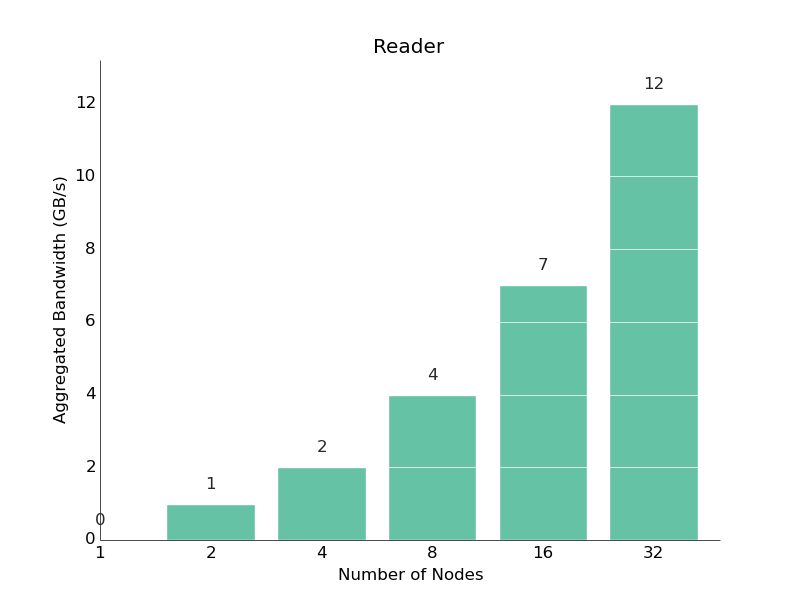
\includegraphics[scale=0.5]{Figures/reader.png}
    \rule{25em}{0.5pt}
  \caption[Generated sample plot]{Generated sample plot}
  \label{fig:plot}
\end{figure}

The current way of benchmarking an MTC filesystem is to write a number of scripts, then use SSH to distribute them across the nodes. Finally, after the scripts are in place, there needs to be another
script that iterates through all the nodes and triggers the benchmarks as close to simultaneously as possible over SSH. This requires a considerate amount of work and there is no true coordination in place, as there is no synchronization method (like the barrier in our solution) to enforce the same start time for the benchmark across all nodes. If at some later time a new test case has to be run, all scripts have to be modified to account for the change.

In contrast, using our project to run the same set of benchmarks, there is only one command to execute, as we have shown. Furthermore, coordination is built-in, thanks to the MPI runner, so we can be certain that all nodes start at the same time. If at some later time a new test case has to be run, it is only a matter of specifying it using our JSON format and the benchmark will keep working. Aside from just running the tests, our solution also includes processing the outputs into machine-readable form, as well as plotting the results.
